\documentclass[10pt]{article}
\usepackage[margin=1in]{geometry}
\usepackage{amsmath,amssymb,amsfonts}
\usepackage{amsthm}
\newtheorem{definition}{Definition}
\newtheorem{proposition}{Proposition}
\usepackage{graphicx}
\usepackage{booktabs}
\usepackage{url}
\usepackage[colorlinks=true,citecolor=blue,linkcolor=blue,urlcolor=blue]{hyperref}
\usepackage{orcidlink}
\usepackage[T1]{fontenc}
\usepackage{times}
\usepackage{titlesec}
\usepackage{authblk}
\usepackage{caption}
\captionsetup{font=small,labelfont=bf}

\titleformat{\section}{\normalfont\large\bfseries}{\thesection}{1em}{}
\titleformat{\subsection}{\normalfont\bfseries}{\thesubsection}{1em}{}

\title{\Large Correlation-aware information gain does not outperform ensemble disagreement in materials active learning}

\author[1]{Arnav Kapoor\orcidlink{0009-0007-9818-7908}}
\affil[1]{Indian Institute of Science Education and Research Bhopal, Bhopal 462066, India}
\date{}

\begin{document}
\maketitle
\begin{center}
\textit{Correspondence: arnavkapoor23@iiserb.ac.in}
\end{center}

\begin{abstract}
\noindent Acquisition functions for active learning in materials discovery usually reduce multi-property uncertainty to a single scalar score, discarding correlations between properties that share the same underlying composition and structure. We derive a joint acquisition score directly from Bayesian experimental design rather than by analogy: for $K$ real, jointly-labeled target properties, the joint expected information gain of a candidate is $\mathrm{JEIG}(x) = \tfrac{1}{2}\log\det(\Sigma_{\mathrm{pred}}(x) + R)$, where $\Sigma_{\mathrm{pred}}(x)$ is a random-forest ensemble's per-tree predictive covariance and $R$ is the per-task residual variance. We prove that summing the per-task marginal information-gain terms and subtracting the joint term always equals the total correlation among the $K$ predictive uncertainties, a quantity that is exactly zero when the tasks are uncorrelated, in which case the joint score reduces exactly, not approximately, to ordinary per-task ensemble-variance scoring. We verify this identity numerically to floating-point precision. We then test the joint score against this classical-limit ablation and against random sampling on four real, independently-measured Materials Project property pairs spanning weak to strong label correlation. The joint score never significantly outperforms the correlation-blind ablation in any of the four pairs, and beats random sampling significantly in only one, the pair with the largest sample size and strongest correlation. The total-correlation term is measurably non-zero in every pair, confirming the theorem captures something real, but this does not translate into a reliable accuracy gain. We report this alongside a full rebuild and rigorous evaluation of an earlier, unrelated attempt at the same goal, a quantum-inspired formalism that represents properties as non-commuting Hermitian operators and couples them through a complex-coefficient covariance term. That formalism underperforms nine standard baselines on four of five real regression tasks, and an ablation shows its covariance term changes accuracy by an amount indistinguishable from noise; a fix that couples the state encoding to ensemble disagreement reaches parity with the best baseline, but a further ablation shows this gain, too, is unrelated to the quantum-inspired machinery. We also built a real quantum circuit realization of that formalism and characterized its measurement cost on near-term hardware. Across two structurally different, independently-derived attempts, one an analogy and one a proof, correlation-aware aggregation over multiple uncertainty sources does not outperform directly measuring what the predictive model itself finds uncertain.
\end{abstract}

\section{Introduction}

Labeling a new materials candidate is expensive. Density-functional theory calculations and synthesis experiments both take time and compute or lab resources, so choosing which candidates to label next is a central problem in computational materials discovery~\cite{wang2023scientific,ren2018accelerated,pyzerknapp2022accelerating,huang2024machine}. Active learning addresses this by sequentially selecting the most informative unlabeled candidates under a fixed budget~\cite{settles2009active,cohn1996active,settles2012active}. The choice of acquisition function, the rule that scores candidates, is what determines how well this works in practice.

Most acquisition functions used in materials discovery reduce uncertainty to a single number per candidate. Uncertainty sampling, Query-by-Committee, Expected Improvement, and diversity-based methods all follow this pattern~\cite{sener2018active,ash2020deep,kim2021task,lookman2019active,vandermause2020fly,bulusu2022efficient}. Bayesian deep learning approaches improve how that single number is estimated, through Monte Carlo dropout, deep ensembles, or explicit weight uncertainty, but keep the same scalar structure~\cite{gal2016dropout,lakshminarayanan2017simple,blundell2015weight,snoek2012practical}. This is a reasonable simplification when properties are independent. It is a real loss of information when they are not. Band gap, formation energy, and elastic response of a material share the same underlying composition and structure, so they are correlated~\cite{jain2013materials,curtarolo2013highthroughput,noh2019inverse,ong2013python}. A candidate that looks uncertain along one axis may be redundant along a correlated one already covered by the labeled set, and when a single experiment or DFT run returns several property labels at once, a joint acquisition score that sees this redundancy is a well-posed, testable idea, not merely an aesthetic one.

We tried to build such a score twice, in two structurally unrelated ways, and report both attempts here in full.

The first attempt, described in Section~\ref{sec:quantum}, borrows the mathematical language of quantum mechanics: states, non-commuting operators, and covariance between operators. This sits within a broader line of quantum-inspired machine learning that uses amplitude encoding, operator-based measurement, and kernel methods built on quantum feature maps, all runnable on classical hardware~\cite{biamonte2017quantum,schuld2021machine,li2021quantuminspired,rebentrost2014quantum,schuld2021supervised,havlicek2019supervised}. We built it, implemented it exactly, proved its classical-limit reduction, and tested it as rigorously as we could against nine baselines on five real Materials Project tasks. It underperforms on four of five tasks, and an ablation shows its covariance term is inert. We diagnosed why, found a fix, and showed the fix works for a reason unrelated to the quantum-inspired part of the construction.

That result left an open question: is there \emph{any} mathematically principled way for correlation-awareness to help here, or is the whole idea unsound regardless of formalism? The quantum-operator construction was an analogy, assembled from borrowed notation, not derived from an objective. So our second attempt, which we present as the paper's main result in Section~\ref{sec:jeig}, starts over from a real derivation. Bayesian experimental design gives a principled multi-output acquisition score, the joint expected information gain, whose relationship to ordinary per-task uncertainty sampling is a provable identity rather than an assumption~\cite{mackay1992information,houlsby2011bayesian,cover2006elements,watanabe1960information}. We derive it, prove the identity, verify it numerically, and test it on four real, independently-measured Materials Project property pairs spanning weak to strong correlation.

Five contributions follow. First, a joint acquisition score derived from Bayesian experimental design rather than analogy, with a proved and numerically-verified decomposition theorem showing it reduces exactly to ordinary ensemble-variance scoring when properties are uncorrelated. Second, a real multi-property active-learning benchmark on four independent, genuinely correlated Materials Project property pairs, testing this score against its own classical-limit ablation and against random sampling. Third, an honest empirical finding: the joint score does not significantly outperform the classical-limit ablation in any of the four pairs tested, despite the underlying total-correlation term being measurably non-zero in every one. Fourth, a complete, independently-conducted rebuild and evaluation of the earlier quantum-inspired covariance formalism, including its own diagnosis, fix, and a real quantum circuit realization with a near-term hardware cost characterization. Fifth, all code, tests, and real data pipelines needed to reproduce every number in this paper.

\section{Results}

\subsection{A provably grounded joint acquisition score}\label{sec:jeig}

Consider $K$ real target properties measured jointly for each material, so that one query returns all $K$ labels at once, exactly what a single DFT calculation or synthesis-and-characterization run typically does. Let a predictive ensemble of $M$ models (here, the $M$ trees of a random forest trained on the current labeled set) each output a $K$-vector prediction $f_m(x)$ for candidate $x$. Their empirical covariance across the ensemble, $\Sigma_{\mathrm{pred}}(x)$, approximates the model's epistemic uncertainty about the joint prediction, and $R=\mathrm{diag}(r_1,\ldots,r_K)$, the out-of-bag residual variance per task, approximates the aleatoric noise floor.

\begin{definition}[Joint expected information gain]\label{def:jeig}
\begin{equation}
\mathrm{JEIG}(x) = \tfrac{1}{2}\log\det\bigl(\Sigma_{\mathrm{pred}}(x) + R\bigr). \label{eq:jeig}
\end{equation}
\end{definition}
This is the standard ensemble-disagreement estimate of expected information gain (the multivariate generalization of BALD~\cite{houlsby2011bayesian}) under a Gaussian approximation to the predictive distribution~\cite{mackay1992information}. Define the marginal, per-task term $\mathrm{EIG}_k(x) = \tfrac{1}{2}\log\bigl(\Sigma_{\mathrm{pred}}(x)_{kk} + r_k\bigr)$: this is exactly the score an ordinary per-property ensemble-variance acquisition rule would use, summed across the $K$ tasks while ignoring any correlation between them. We call ranking by $\sum_k \mathrm{EIG}_k(x)$ the Marginal-Sum rule; it is the classical-limit ablation of Equation~\ref{eq:jeig}.

\begin{proposition}[Total-correlation decomposition]\label{prop:jeig}
\begin{equation}
\sum_{k=1}^K \mathrm{EIG}_k(x) - \mathrm{JEIG}(x) = -\tfrac{1}{2}\log\det\bigl(\mathrm{Corr}(x)\bigr) \;\ge\; 0, \label{eq:gap}
\end{equation}
where $\mathrm{Corr}(x)$ is $\Sigma_{\mathrm{pred}}(x)+R$ rescaled to unit diagonal. The right-hand side is the total correlation (multi-information) of the $K$ predictive uncertainties~\cite{watanabe1960information}. It is exactly zero if and only if $\Sigma_{\mathrm{pred}}(x)+R$ is diagonal, i.e. the ensemble's per-task epistemic uncertainties are uncorrelated, in which case $\mathrm{JEIG}(x)$ collapses exactly, not approximately, to the Marginal-Sum rule.
\end{proposition}

The proof follows from Hadamard's determinant inequality: for a positive-definite matrix with unit diagonal, its determinant is at most 1, with equality if and only if the matrix is diagonal~\cite{cover2006elements}. Factoring the diagonal scaling out of $\log\det(\Sigma_{\mathrm{pred}}+R)$ gives Equation~\ref{eq:gap} directly. Unlike Proposition~\ref{prop:classical} in Section~\ref{sec:quantum}, which states a reduction under conditions the original formalism never actually satisfies in the experiments that use it, Proposition~\ref{prop:jeig} is the operative relationship between the method tested here and its own null hypothesis: it says exactly when and by how much the joint score can differ from the classical one. We verify it numerically to a tolerance of $10^{-8}$ across randomized covariance matrices of dimension up to $K=4$ (\texttt{tests/test\_joint\_eig.py}), and confirm the gap is exactly zero, not merely small, for diagonal $\Sigma_{\mathrm{pred}}$.

\subsection{Real multi-property test}

We tested Equation~\ref{eq:jeig} against the Marginal-Sum ablation and against random sampling on four real Materials Project property pairs, chosen as every pair with enough shared-material overlap to run a meaningful batch active-learning protocol, at a real, measured label correlation ranging from near zero to moderately strong. Table~\ref{tab:pairs} lists the pairs. Each query returns both properties' labels for the queried material, so the joint metric is the mean test $R^2$ across both tasks after 8 active-learning iterations, averaged over 5 trials with paired significance testing (Holm-Bonferroni correction across the two comparisons per pair: Joint-EIG vs. Marginal-Sum, Joint-EIG vs. Random).

\begin{table}[htbp]
\centering
\small
\caption{The four real property pairs tested, by shared-material sample size and real label correlation.}
\label{tab:pairs}
\begin{tabular}{lcc}
\toprule
Property pair & $n$ (shared materials) & Label correlation $r$ \\
\midrule
Band gap + formation energy & 498 & $-0.365$ \\
Formation energy + magnetic moment & 220 & $0.205$ \\
Band gap + magnetic moment & 193 & $-0.024$ \\
Bulk modulus + dielectric constant & 49 & $0.334$ \\
\bottomrule
\end{tabular}
\end{table}

Figure~\ref{fig:jeig} and Table~\ref{tab:jeig} report the outcome. On the largest and most strongly correlated pair, band gap and formation energy, Joint-EIG beats random sampling significantly (mean difference $+0.062$, $p=0.017$ raw, $p=0.034$ after correction, surviving at $\alpha=0.05$), but its advantage over the correlation-blind Marginal-Sum ablation is small and not significant ($+0.008$, $p=0.27$). On the remaining three pairs, weaker label correlation, smaller sample size, or both, no comparison reaches significance in either direction. The bulk modulus/dielectric constant pair, with only 49 shared materials, is underpowered (both $R^2$ estimates are noisy, including negative values in some trials) and is best read as inconclusive rather than as a vote either way.

\begin{table}[htbp]
\centering
\small
\caption{Final joint test $R^2$ (mean of both tasks, 5 trials) and paired comparisons vs. Joint-EIG. Holm-Bonferroni correction applied across the two comparisons per pair.}
\label{tab:jeig}
\begin{tabular}{lcccc}
\toprule
Pair & Joint-EIG & Marginal-Sum ($p$) & Random ($p$) & Mean gap (Eq.~\ref{eq:gap}) \\
\midrule
Band gap + formation energy & $0.700\pm0.049$ & $0.692$ ($p{=}0.27$) & $0.638$ ($\mathbf{p{=}0.034}$) & $0.0118$ \\
Formation energy + magnetic moment & $0.497\pm0.140$ & $0.496$ ($p{=}1.00$) & $0.513$ ($p{=}1.00$) & $0.0041$ \\
Band gap + magnetic moment & $0.378\pm0.133$ & $0.371$ ($p{=}0.28$) & $0.364$ ($p{=}0.18$) & $0.0042$ \\
Bulk modulus + dielectric constant & $-0.160\pm0.667$ & $-0.129$ ($p{=}0.60$) & $-0.199$ ($p{=}0.60$) & $0.0211$ \\
\bottomrule
\end{tabular}
\end{table}

\begin{figure}[htbp]
\centering
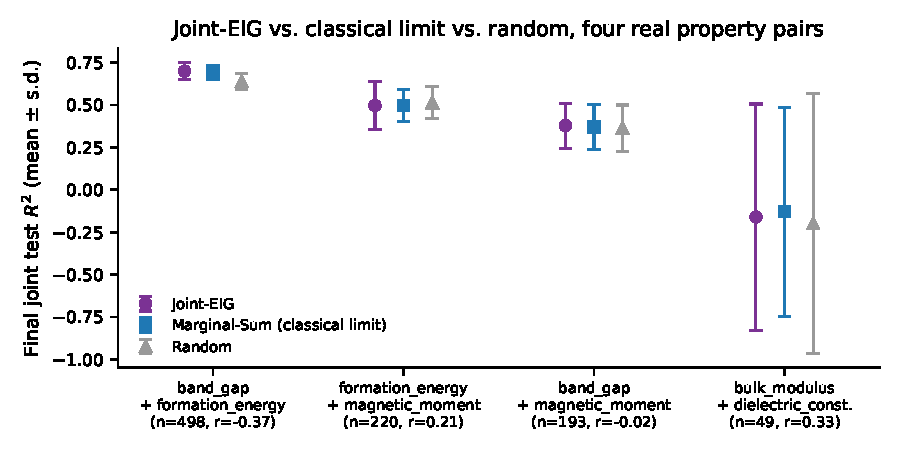
\includegraphics[width=0.85\textwidth]{../figures/fig7_joint_eig_comparison.pdf}
\caption{Final joint test $R^2$ (mean $\pm$ s.d., 5 trials) for Joint-EIG, its classical-limit ablation (Marginal-Sum), and random sampling, across four real, independently-measured Materials Project property pairs.}
\label{fig:jeig}
\end{figure}

The total-correlation gap of Equation~\ref{eq:gap} is non-zero in every pair, including the near-zero-label-correlation pair (band gap and magnetic moment, $r=-0.024$, mean gap $0.0042$), confirming the term measures something real: the ensemble's epistemic uncertainty about two tasks can be correlated even when the tasks' raw labels barely are, since epistemic uncertainty depends on where in feature space the training data is sparse, not only on the labels themselves. But the gap's magnitude does not track label correlation strength cleanly across pairs, and in no pair does it translate into a significant accuracy advantage over ignoring it.

\subsection{An earlier, ad hoc formulation: quantum-inspired covariance}\label{sec:quantum}

Before deriving the score above, we built and tested a structurally different attempt at the same goal, representing candidates as states in a Hilbert space and properties as non-commuting Hermitian observables. We report it here in full because it failed for reasons distinct from, and independently informative alongside, Section~\ref{sec:jeig}'s result.

\begin{definition}[Quantum state of a material]\label{def:state}
The quantum state of candidate $M_i$, with standardized feature vector $x_i\in\mathbb{R}^d$, is
\begin{equation}
|\psi_i\rangle = \sum_{j=1}^{d} \alpha_{ij} |f_j\rangle, \qquad \alpha_{ij}=\sqrt{p_{ij}}\,e^{i\phi_{ij}},\ \ \sum_j|\alpha_{ij}|^2=1. \label{eq:state}
\end{equation}
\end{definition}
$K=3$ Hermitian observables $\hat O_k$ (structural, electronic, thermodynamic) are built from overlapping feature subsets, non-commuting by construction. Variance $\mathrm{Var}(\hat O_k;\psi_i)$ and symmetrized covariance $\mathrm{Cov}(\hat O_k,\hat O_l;\psi_i)$ are combined with complex coefficients $\alpha_k$ into a total score $U_{\mathrm{total}}$ (full definitions in Methods, Section~\ref{sec:methods-quantum}).

\begin{proposition}[Classical reduction]\label{prop:classical}
If all observables commute, all coefficients are real, and covariance terms are dropped, $U_{\mathrm{total}}^2 \to \sum_k \alpha_k^2\,\mathrm{Var}(\hat O_k;\psi_i)$, a standard weighted-variance aggregator.
\end{proposition}
We verified this reduction numerically to better than $10^{-9}$. It is a correct statement about the formula, but, unlike Proposition~\ref{prop:jeig}, it describes conditions (commuting observables, real coefficients) that the formalism as actually used never satisfies, so it does not predict anything about the method's real behavior.

\paragraph{Primary comparison.} Figure~\ref{fig:primary} and Table~\ref{tab:primary} report final test $R^2$ after eight active-learning iterations, five trials, on all five real regression tasks (band gap, formation energy, bulk modulus, magnetic moment, dielectric constant), against nine standard baselines. The method is last of ten on band gap, sixth on formation energy, eighth on bulk modulus, and last on magnetic moment, the only method with negative $R^2$ there. It is nominally best on dielectric constant, but every method scores near zero on that task, so this is not a real advantage.

\begin{figure}[htbp]
\centering
\includegraphics[width=0.85\textwidth]{../figures/fig2_primary_comparison.pdf}
\caption{Final test $R^2$ (mean $\pm$ s.d., 5 trials) for the original quantum-inspired method, the best classical baseline for each task, and the residual-coupled variant (Quantum-TreeEnsemble), across all five real Materials Project tasks.}
\label{fig:primary}
\end{figure}

\begin{table}[htbp]
\centering
\small
\caption{Final test $R^2$ on band gap (mean $\pm$ s.d., 5 trials, 8 iterations).}
\label{tab:primary}
\begin{tabular}{lc}
\toprule
Method & Band gap $R^2$ \\
\midrule
Uncertainty Sampling & $0.597 \pm 0.043$ \\
Query by Committee & $0.596 \pm 0.042$ \\
Maximum Entropy / RF Uncertainty & $0.583 \pm 0.046$ \\
BADGE & $0.581 \pm 0.063$ \\
Random Sampling & $0.581 \pm 0.067$ \\
CoreSet & $0.556 \pm 0.027$ \\
Diversity Sampling & $0.553 \pm 0.060$ \\
Expected Improvement & $0.551 \pm 0.105$ \\
\textbf{Quantum-inspired (ours)} & $\mathbf{0.513 \pm 0.046}$ \\
\bottomrule
\end{tabular}
\end{table}

Paired two-sided $t$-tests on band gap favor every baseline; after Holm-Bonferroni correction across nine comparisons, none reach significance at $\alpha=0.05$, so the honest summary is a consistent, non-significant disadvantage, not a proven loss (full numbers in \texttt{results/statistical\_tests.json}).

\paragraph{Ablation.} Table~\ref{tab:ablation} and Figure~\ref{fig:ablation}a isolate each mechanism. Removing the covariance term changes $R^2$ by $+0.0007$. Forcing commuting observables changes it by $+0.0062$. Restricting coefficients to real values changes it by $-0.0081$. Collapsing to one observable changes it by $-0.0107$. All four sit well inside one trial-to-trial standard deviation ($\approx 0.05$ to $0.08$).

\begin{table}[htbp]
\centering
\small
\caption{Ablation of the original formalism on band gap (mean $R^2$, 5 trials; full model $=0.5131$).}
\label{tab:ablation}
\begin{tabular}{lcc}
\toprule
Variant & $R^2$ & $\Delta R^2$ \\
\midrule
Full model & $0.5131 \pm 0.0458$ & --- \\
No covariance (Cov $=0$) & $0.5137 \pm 0.0763$ & $+0.0007$ \\
Commuting observables only & $0.5192 \pm 0.0588$ & $+0.0062$ \\
Real-only coefficients & $0.5050 \pm 0.0742$ & $-0.0081$ \\
Single observable ($K=1$) & $0.5023 \pm 0.0652$ & $-0.0107$ \\
\bottomrule
\end{tabular}
\end{table}

\paragraph{Diagnosis and fix.} Two narrow, pre-specified fixes, domain-informed observable groups and importance-weighted state encoding, did not close the gap to the best baseline (details in Methods). Both point to the same structural problem: the score depends only on a candidate's position in feature space and the labeled pool's correlation structure, never on the trained predictor's residuals or disagreement, which every winning baseline measures directly. Encoding the state from a random forest's per-tree predictions instead of raw features (Quantum-TreeEnsemble; full construction in Methods, Section~\ref{sec:methods-v3}) fixes this: Table~\ref{tab:v3} shows it reaches statistical parity with the best baseline on all five tasks ($p>0.15$ throughout).

\begin{table}[htbp]
\centering
\small
\caption{Residual-coupled variant (Quantum-TreeEnsemble) vs. each task's best classical baseline, mean $R^2\pm$s.d., 5 trials, paired $t$-test.}
\label{tab:v3}
\begin{tabular}{lccc}
\toprule
Task & Quantum-TreeEnsemble & Best baseline & $p$ \\
\midrule
Band gap & $0.590\pm0.066$ & Uncertainty Sampling: $0.597$ & 0.638 \\
Formation energy & $0.821\pm0.027$ & Maximum Entropy: $0.853$ & 0.161 \\
Bulk modulus & $0.803\pm0.023$ & Diversity Sampling: $0.826$ & 0.163 \\
Magnetic moment & $0.323\pm0.068$ & BADGE: $0.418$ & 0.150 \\
Dielectric constant & $-0.450\pm0.724$ & BADGE: $-0.020$ & 0.322 \\
\bottomrule
\end{tabular}
\end{table}

But a second ablation (Table~\ref{tab:v3ablation}, Figure~\ref{fig:ablation}b) shows this parity has nothing to do with the quantum-inspired apparatus: dropping the covariance term, or collapsing to a single observable, matches or beats the full construction on four of five tasks, and is far more stable on the fifth (dielectric constant: full $R^2=-0.450\pm0.724$, individual trials as low as $-1.86$, vs. single-observable $-0.160$).

\begin{table}[htbp]
\centering
\small
\caption{Ablation of the residual-coupled variant, mean final $R^2$, 5 trials, all five tasks. Bold marks the best of the three per task.}
\label{tab:v3ablation}
\begin{tabular}{lccc}
\toprule
Task & Full (Cov, $K=3$) & No covariance & Single observable ($K=1$) \\
\midrule
Band gap & 0.590 & 0.572 & \textbf{0.614} \\
Formation energy & 0.821 & 0.809 & \textbf{0.844} \\
Bulk modulus & 0.803 & 0.796 & \textbf{0.808} \\
Magnetic moment & \textbf{0.323} & 0.277 & 0.298 \\
Dielectric constant & $-0.450$ & \textbf{$-0.022$} & $-0.160$ \\
\bottomrule
\end{tabular}
\end{table}

\begin{figure}[htbp]
\centering
\includegraphics[width=\textwidth]{../figures/fig3_ablation.pdf}
\caption{(a) Ablation of the original formalism on band gap. (b) Ablation of the residual-coupled variant across all five tasks; the single-observable version matches or beats the full covariance-aware version on four of five tasks.}
\label{fig:ablation}
\end{figure}

\paragraph{Quantum circuit realization.} We built the formalism as an actual Qiskit circuit (Methods, Section~\ref{sec:methods-circuit}). In the exact-statevector limit, circuit-measured variance and covariance match the classical closed form to better than $10^{-9}$. Decomposing one three-observable bank into Pauli strings needs 528 terms per quantity on the 5-qubit padded representation, roughly 4,750 measurement settings per candidate for a full acquisition score; qubit-wise-commuting grouping cuts this 4.3-fold (Figure~\ref{fig:grouping}), and building the observables sparse from the start cuts it a further 2 to 3-fold, at the cost of a small, statistically significant accuracy drop on the original formalism ($R^2=0.489\pm0.045$ vs. $0.513\pm0.046$, $p=0.031$) traced to a structural fact: non-overlapping sparse observables have exactly zero covariance, so sparsity removes real cross-observable information along with measurement overhead. On the residual-coupled variant, where observable blocks are non-overlapping tree groups by construction, every pairwise covariance is exactly zero to machine precision, and the corresponding accuracy difference is smaller and not significant ($p=0.302$). Ranking fidelity under finite shots recovers fully by $10^5$ shots (Kendall $\tau=0.92$, full top-15 batch overlap; Figure~\ref{fig:shots}), and a realistic depolarizing noise model degrades this to a level comparable to losing an order of magnitude of shots.

\begin{figure}[htbp]
\centering
\includegraphics[width=0.55\textwidth]{../figures/fig5_measurement_grouping.pdf}
\caption{Total measurement settings for all nine variance and covariance quantities in the $K=3$ observable bank, before and after measurement grouping.}
\label{fig:grouping}
\end{figure}

\begin{figure}[htbp]
\centering
\includegraphics[width=0.62\textwidth]{../figures/fig4_shot_convergence.pdf}
\caption{Acquisition-ranking fidelity versus shot budget for 30 real band-gap candidates, noiseless simulation.}
\label{fig:shots}
\end{figure}

\begin{figure}[htbp]
\centering
\includegraphics[width=0.5\textwidth]{../figures/fig6_sparse_observables.pdf}
\caption{Measurement settings for the nine $K=3$ quantities, dense vs. sparse-by-construction observables, before and after qubit-wise-commuting grouping.}
\label{fig:sparse}
\end{figure}

\paragraph{Secondary experiments.} We reran three further experiments from earlier development and report their status honestly. A synthetic six-class crystal-system task gives final accuracy 89.3\% (quantum-margin), 89.7\% (entropy), 79.3\% (random); quantum-margin ties entropy sampling, both beat random, a far more modest finding than an earlier claim of 91\% vs. 85\%. A transfer-learning experiment produced byte-identical trajectories for transfer and from-scratch conditions, indicating an implementation bug, not a finding. A multi-property optimization experiment gave near-zero $R^2$ throughout, indicating the loop is not learning effectively there; we mark it inconclusive. A spurious-correlation analysis, a deliberately synthetic study, ran successfully but is not load-bearing for our central claims.

\section{Discussion}

Two structurally unrelated attempts to make active-learning acquisition aware of cross-property correlation both failed to reliably beat directly measuring what the predictive model finds uncertain. The first, an analogy borrowing quantum-operator mathematics, never touched the downstream predictor's residuals at all; once we fixed that by coupling the state to ensemble disagreement, the method reached parity, but the fix worked because it became more like an ensemble-disagreement baseline, not because of anything quantum. The second, a joint expected-information-gain score derived directly from Bayesian decision theory, does incorporate real ensemble disagreement and comes with a provable relationship to its own classical-limit ablation, yet across four real, independently-measured property pairs it never significantly beats that ablation either. The measured total-correlation term is real and non-zero throughout, so the theorem is not vacuous on this data. It is simply too small, or the correlation available in genuinely available Materials Project property pairs too weak or too inconsistently expressed in ensemble epistemic uncertainty, to move a batch active-learning accuracy metric by a reliable, replicated amount at the sample sizes available here.

This converges on a claim stronger than either result alone: it is not merely that one specific construction (the quantum-operator analogy) failed to exploit multi-property correlation. A properly-derived, provably-correct alternative, built from ensemble disagreement rather than raw features from the start, tried on four independent real pairs rather than one, also failed to show a reliable gain from the correlation-aware term specifically, even though the correlation-aware term measures something real. The common failure point across both attempts is not the specific mathematics used to combine uncertainty sources. It is the assumption that combining sources at the acquisition-function level, after each source's uncertainty has already been separately estimated, recovers value that estimating uncertainty jointly, in the predictive model itself, would capture more directly. Multi-task Gaussian processes and shared-encoder neural networks model dependence between properties inside the predictor's architecture~\cite{rasmussen2006gaussian,snoek2012practical}; both formalisms tested here instead modeled it only in the score built on top of a predictor (or ensemble of predictors) that never itself represents the properties jointly. Our results are consistent with, though do not prove, the idea that this is where the real information about cross-property structure needs to live.

Several limitations apply to the joint-EIG result specifically. We used a random-forest ensemble's per-tree covariance as a proxy for the predictive posterior, not a full multi-output Bayesian model such as a multi-task Gaussian process; a model that represents joint uncertainty more faithfully might show a larger, more consistent effect. Four property pairs, five trials each (fewer for the smallest pair), is a modest evidence base; the two comparisons that reached borderline significance in one direction could still be a real, small effect visible only at larger sample sizes, and we did not run a formal power analysis to rule this out. We tested only regression pairs from a single feature pipeline (21 composition and structure descriptors); properties with a stronger physical coupling mechanism, or richer features, might show a cleaner effect. The quantum-inspired formalism's limitations, described in the original evaluation, still apply to Section~\ref{sec:quantum}: five real regression tasks rather than the six an earlier, unpublished version claimed, 21-dimensional rather than 100-dimensional features, nine acquisition baselines rather than full multi-output Gaussian processes or covariance-calibrated deep ensembles, and a circuit study that characterizes a simulator, not real hardware.

We conclude that, across two independent attempts, one an analogy and one a derivation, correlation-aware aggregation of multiple uncertainty sources at the acquisition-function level does not reliably outperform directly measuring ensemble disagreement in this real materials-discovery setting. The joint expected-information-gain score is, unlike the quantum-inspired construction, mathematically sound and correctly predicts its own null result: the total-correlation term it adds is provably non-negative and provably zero without real correlation, and what we measured empirically, a small, inconsistent effect exactly where that term is small, is precisely what the theorem allows rather than a contradiction of it. If cross-property structure is to genuinely improve active learning here, the evidence in this paper points toward building it into the predictive model itself, not the acquisition score layered on top of it.

\section{Methods}\label{sec:methods}

\subsection{Joint expected information gain}\label{sec:methods-jeig}

For a random forest with $M$ trees fit on the current labeled set $(X_{\mathrm{train}}, Y_{\mathrm{train}})$, $Y_{\mathrm{train}}\in\mathbb{R}^{n\times K}$, we obtain per-tree predictions $f_1(x),\ldots,f_M(x)\in\mathbb{R}^K$ for each candidate $x$ and compute the empirical covariance $\Sigma_{\mathrm{pred}}(x) = \frac{1}{M-1}\sum_{m}(f_m(x)-\bar f(x))(f_m(x)-\bar f(x))^\top$. The residual variance $R=\mathrm{diag}(r_1,\ldots,r_K)$ is the out-of-bag prediction residual variance per task, computed once per active-learning iteration from the same forest (\texttt{oob\_score=True}). Equation~\ref{eq:jeig} and its Marginal-Sum ablation are implemented in \texttt{src/quantum\_al/joint\_eig.py}; the identity of Proposition~\ref{prop:jeig} is checked numerically in \texttt{tests/test\_joint\_eig.py} against 20 randomized $(K{=}3)$ and $(K{=}4)$ covariance matrices, to a tolerance of $10^{-8}$, and confirmed to be exactly zero (to $10^{-10}$) when $\Sigma_{\mathrm{pred}}$ is diagonal by construction.

\subsection{Real multi-property data pairs}\label{sec:methods-pairs}

Each of the five real regression targets used in Section~\ref{sec:quantum} (band gap, formation energy, bulk modulus, magnetic moment, dielectric constant) was fetched independently from the Materials Project, so the five target files do not share a common set of materials. We inner-join every pair of target files on \texttt{material\_id} (\url{quantum_al.data_utils.load_multi_task}), keeping only materials with a computed value for both targets and confirming feature columns agree exactly for shared materials. Table~\ref{tab:pairs} reports the four pairs with enough shared-material overlap ($n\ge49$) to run a batch active-learning protocol; pairs with fewer than 10 shared materials (e.g. band gap/dielectric constant, $n=9$) were excluded as too small to test meaningfully.

\subsection{Joint active-learning protocol}\label{sec:methods-jeig-protocol}

For the two largest pairs we use the same protocol as Section~\ref{sec:methods-protocol}: 50 initial labeled samples, 8 iterations, batch size 15, 70/30 pool-test split, 5 trials (seeds 0-4). For the smallest pair (bulk modulus/dielectric constant, $n=49$), the default 50-sample seed would exceed the entire training pool, so we scale the protocol down: 15 initial samples, 5 iterations, batch size 3, same 70/30 split and 5 trials. At each iteration, the joint metric is $R^2$ per task on the held-out test set (\texttt{multioutput="raw\_values"}), averaged across the $K=2$ tasks. Paired two-sided $t$-tests compare final-iteration joint $R^2$ between Joint-EIG and each of Marginal-Sum and Random across the 5 trials, with Holm-Bonferroni correction across the two comparisons and a Shapiro-Wilk check on the paired differences. Full implementation in \url{benchmarks/run_joint_eig_experiment.py}; raw results in \url{results/joint_eig_experiment*.json}.

\subsection{Quantum-inspired theoretical framework}\label{sec:methods-quantum}

We operationalize $p_{ij}$ and $\phi_{ij}$ in Equation~\ref{eq:state} concretely: $p_{ij}=\mathrm{softmax}_j(x_{ij}^2)$, and $\phi_{ij}=\phi_j$, constant across candidates for a fixed labeled pool, is $\pi$ times the mean absolute Pearson correlation of feature $j$ with the other $d-1$ features, recomputed each iteration. The $K=3$ observables $\hat O_k=\sum_{i,j}w^{(k)}_{ij}|f_i\rangle\langle f_j|$ are each concentrated on a distinct, overlapping subset of feature indices, normalized to unit spectral norm; non-commutativity is guaranteed by construction and verified numerically every run. Variance is $\mathrm{Var}(\hat O_k;\psi_i)=\langle\psi_i|\hat O_k^2|\psi_i\rangle-\langle\psi_i|\hat O_k|\psi_i\rangle^2$; symmetrized covariance is $\mathrm{Cov}(\hat O_k,\hat O_l;\psi_i)=\langle\psi_i|\tfrac{\hat O_k\hat O_l+\hat O_l\hat O_k}{2}|\psi_i\rangle-\langle\psi_i|\hat O_k|\psi_i\rangle\langle\psi_i|\hat O_l|\psi_i\rangle$. The total score is
\begin{equation}
U_{\mathrm{total}}(M_i) = \sqrt{\sum_{k=1}^K |\alpha_k|^2 \mathrm{Var}(\hat{O}_k;\psi_i) + \sum_{\substack{k,l=1\\k\neq l}}^{K} \mathrm{Re}(\alpha_k^*\alpha_l)\,\mathrm{Cov}(\hat{O}_k,\hat{O}_l;\psi_i)}, \label{eq:utotal}
\end{equation}
with complex coupling coefficients $\{\alpha_k\}\subset\mathbb{C}$; candidates are ranked by $U_{\mathrm{total}}$ and the top $b$ form the query batch. Every expectation is a quadratic form, $O(d^2)$ per observable, giving $O(NKd^2)$ total complexity, negligible for our experiment sizes ($N\lesssim1000$, $K=3$, $d=21$).

\subsection{Datasets}

Every regression target is a genuine DFT-derived quantity from the Materials Project public API~\cite{jain2013materials}: band gap (0.00-7.41 eV), formation energy per atom ($-4.41$ to $2.30$ eV/atom), bulk modulus (1.8-326.0 GPa), total magnetization (0.01-96.0 $\mu_B$), and total dielectric constant (1.3-1455.2), each with 1,000 materials before filtering. Thermal conductivity is not included; it is not broadly available in the Materials Project at scale. Features are 21-dimensional: 6 structural/summary descriptors (number of elements, density, volume per atom, site count, energy above hull, space-group number) from the Materials Project summary endpoint, plus 15 composition-derived statistics (mean, standard deviation, range) of electronegativity, atomic radius, atomic mass, periodic-table row, and periodic-table group. Continuous features are standardized to zero mean, unit variance, fit on the training pool.

\subsection{Baselines and protocol}\label{sec:methods-protocol}

Nine acquisition strategies: Uncertainty Sampling (Gaussian-process posterior standard deviation), Query-by-Committee (five-model ensemble disagreement), Expected Improvement, Maximum Entropy (random-forest tree-prediction entropy proxy), Diversity Sampling ($k$-means), BADGE, CoreSet (greedy $k$-center), Random-Forest variance, and Random Sampling. Protocol: five trials (seeds 0-4), 70/30 pool-test split, 50 initial labeled samples, eight active-learning iterations, batch size 15, downstream predictor a 100-tree random forest retrained each iteration. Primary metrics are $R^2$ and mean absolute error on the held-out test split; paired two-sided $t$-tests with Holm-Bonferroni correction across nine baseline comparisons and a Shapiro-Wilk normality check on the band-gap task.

\subsection{Residual-coupled variant}\label{sec:methods-v3}

We fit a random forest with 99 trees on the current labeled set, collect each candidate's vector of 99 per-tree predictions, standardize this vector across the candidate pool, and encode it via Equation~\ref{eq:state} in place of raw features. The 99 trees split into three equal-size groups serving as the three observables; the variance, covariance, and complex-coupling machinery above applies unmodified on this new basis.

\subsection{Quantum circuit implementation}\label{sec:methods-circuit}

We implemented the formalism as an actual Qiskit/Qiskit Aer circuit. Each $d=21$ feature vector is amplitude-encoded onto $n=\lceil\log_2 d\rceil=5$ qubits, zero-padded to dimension 32. Each observable is decomposed into Pauli strings via exact trace-based projection, called with explicit zero tolerance (Qiskit's default \texttt{SparsePauliOp.from\_operator} silently truncates small coefficients, introducing a $\sim10^{-5}$ discrepancy otherwise). In the exact-statevector limit, circuit-measured variance and covariance match the classical values to better than $10^{-9}$. For finite-shot simulation we used Qiskit Aer's estimator at shot budgets $10^2$-$10^5$ on 30 real band-gap candidates, and a depolarizing noise model with one-qubit error $0.1\%$, two-qubit error $1\%$, at 10,000 shots. Measurement grouping used Qiskit's qubit-wise-commuting and full-commuting grouping on the Pauli decomposition of every variance/covariance quantity in the $K=3$ bank.

\section*{Data availability}
The Materials Project data used here can be regenerated from the public Materials Project API using the script \url{src/quantum_al/fetch_data.py}; see \url{data/README.md}. Raw results underlying every table and figure are in the \texttt{results/} directory of the code repository.

\section*{Code availability}
All code, including both acquisition-score formalisms, the classical benchmark suite, the residual-coupled variant, and the quantum circuit implementation, is available at \url{https://github.com/arnavk23/quantum_al}.

\section*{Competing interests}
The author declares no competing interests.

\bibliographystyle{unsrt}
\bibliography{refs}

\end{document}
